%%%%%%%%%%%%%%%%%%%%%%%%%%%%%%%%%%%%%%
% Multiplicative domain poster
% Created by Nathaniel Johnston
% August 2009
% http://www.nathanieljohnston.com/2009/08/latex-poster-template/
%%%%%%%%%%%%%%%%%%%%%%%%%%%%%%%%%%%%%%

\documentclass[final]{beamer}
\usepackage[scale=1.24]{beamerposter}
\usepackage{graphicx}			% allows us to import images

%-----------------------------------------------------------
% Custom commands that I use frequently
%-----------------------------------------------------------

\newcommand{\bb}[1]{\mathbb{#1}}
\newcommand{\cl}[1]{\mathcal{#1}}
\newcommand{\fA}{\mathfrak{A}}
\newcommand{\fB}{\mathfrak{B}}
\newcommand{\Tr}{{\rm Tr}}
\newtheorem{thm}{Theorem}

%-----------------------------------------------------------
% Define the column width and poster size
% To set effective sepwid, onecolwid and twocolwid values, first choose how many columns you want and how much separation you want between columns
% The separation I chose is 0.024 and I want 4 columns
% Then set onecolwid to be (1-(4+1)*0.024)/4 = 0.22
% Set twocolwid to be 2*onecolwid + sepwid = 0.464
%-----------------------------------------------------------

\newlength{\sepwid}
\newlength{\onecolwid}
\newlength{\twocolwid}
\setlength{\paperwidth}{48in}
\setlength{\paperheight}{36in}

% % 3 columnm
% \setlength{\sepwid}{0.024\paperwidth}
% \setlength{\onecolwid}{0.3\paperwidth}
% \setlength{\twocolwid}{0.624\paperwidth}

% 4 column
\setlength{\sepwid}{0.024\paperwidth}
\setlength{\onecolwid}{0.22\paperwidth}
\setlength{\twocolwid}{0.464\paperwidth}

\setlength{\topmargin}{-0.5in}
\usetheme{confposter}
\usepackage{exscale}

%-----------------------------------------------------------
% The next part fixes a problem with figure numbering. Thanks Nishan!
% When including a figure in your poster, be sure that the commands are typed in the following order:
% \begin{figure}
% \includegraphics[...]{...}
% \caption{...}
% \end{figure}
% That is, put the \caption after the \includegraphics
%-----------------------------------------------------------

\usecaptiontemplate{
\small
\structure{\insertcaptionname~\insertcaptionnumber:}
\insertcaption}

%-----------------------------------------------------------
% Define colours (see beamerthemeconfposter.sty to change these colour definitions)
%-----------------------------------------------------------

\setbeamercolor{block title}{fg=ngreen,bg=white}
\setbeamercolor{block body}{fg=black,bg=white}
\setbeamercolor{block alerted title}{fg=white,bg=dblue!70}
\setbeamercolor{block alerted body}{fg=black,bg=dblue!10}

%-----------------------------------------------------------
% Name and authors of poster/paper/research
%-----------------------------------------------------------

\title{Spectral Stability of Multi-Pulse Solutions to the Suspension Bridge Equation}
\author{Ross Parker, Bj\"{o}rn Sandstede, Todd Kapitula }
\institute{Division of Applied Mathematics, Brown University \hspace{2in} Department of Mathematics, Calvin College}

%-----------------------------------------------------------
% Start the poster itself
%-----------------------------------------------------------
% The \rmfamily command is used frequently throughout the poster to force a serif font to be used for the body text
% Serif font is better for small text, sans-serif font is better for headers (for readability reasons)
%-----------------------------------------------------------

\begin{document}
\begin{frame}[t]
  \begin{columns}[t]												% the [t] option aligns the column's content at the top
    \begin{column}{\sepwid}\end{column}			% empty spacer column

% first column
    \begin{column}{\onecolwid}
     
      \begin{block}{Suspension Bridge Equation}
          Model for waves on a suspended beam (\cite{Chen97})
            \[ u_{tt} + u_{xxxx} + u^+ - 1 = 0 \]
          Smooth approximation (\cite{Chen97})
            \[ u_{tt} + u_{xxxx} + e^{u} - 1 = 0 \]
          In co-moving frame with speed $c$
            \begin{equation}\label{PDEc}
            u_{tt} - 2 c u_{x t} + u_{xxxx} + c^2 u_{xx} + e^{u} - 1 = 0
            \end{equation}
      \end{block}

      \begin{block}{Homoclinic Orbits}
        \rmfamily{
          Equilibrium solution satisfies ODE
            \begin{equation}\label{eqODE}
             u_{xxxx} + c^2 u_{xx} + e^{u} - 1 = 0
             \end{equation}
          Eigenvalues of linearization about 0, for $c \in (0, \sqrt{2})$
          \vskip0.1ex
          \begin{align*}
          \mu &= \pm \sqrt{\frac{-c^2 \pm \sqrt{c^4 - 4}}{2} } = \pm \alpha \pm \beta i
          \end{align*}
          \vskip1ex
            2D stable manifold, 2D unstable manifold\\
          \vskip1ex
          \textbf{Theorem 1. }(\cite{Berg18}) For $c^2 \in [0.5, 1.9]$, a homoclinic orbit (primary pulse) solution $q(x)$ of \eqref{eqODE} exists which is smooth, even, and decays exponentially to 0 as $x \rightarrow \pm \infty.$
        }
      \end{block}

      \vskip1ex

      \begin{block}{Numerical Construction}
        \rmfamily{

          Primary pulse solutions $q(x)$ constructed numerically using the string method (\cite{Chamard11})

          \begin{figure}
          \begin{center}
          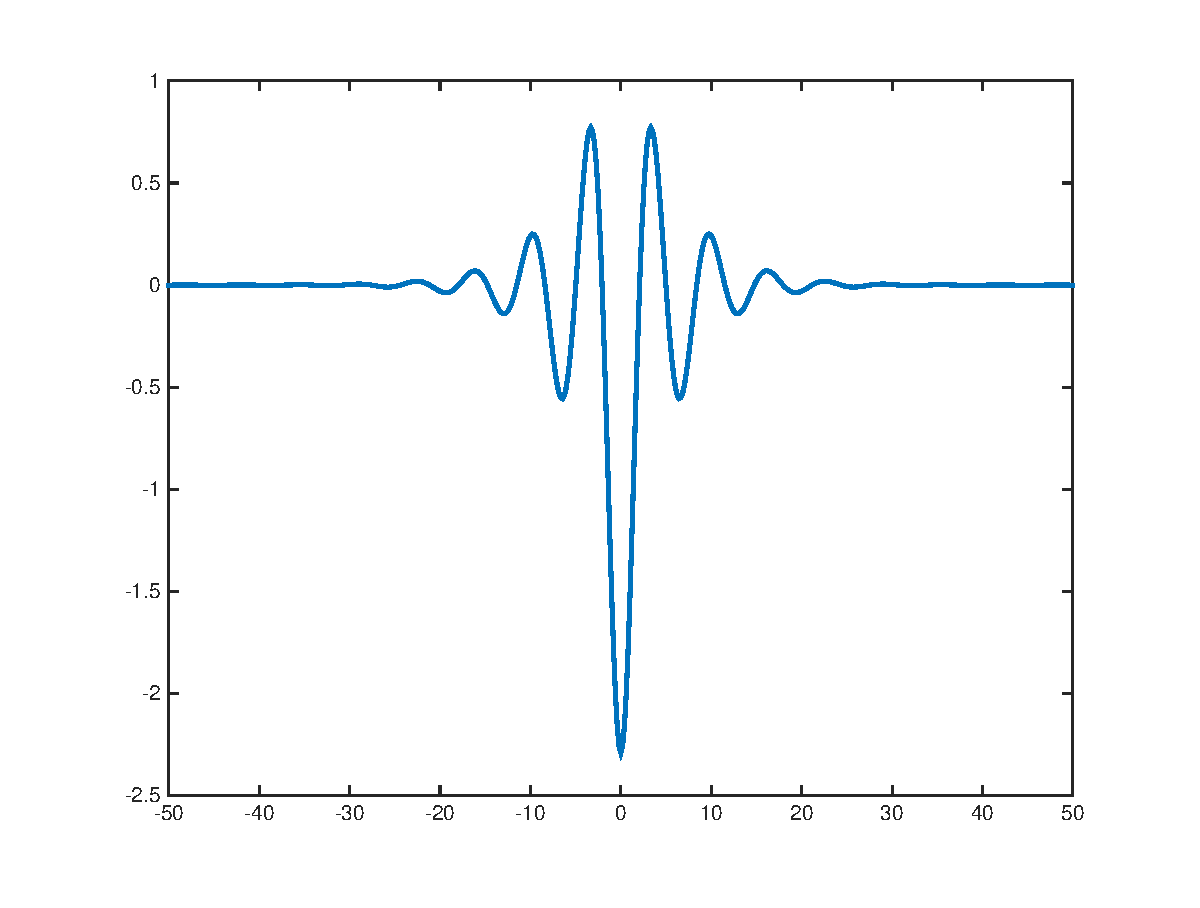
\includegraphics[width=13cm]{images/single1354.eps}
          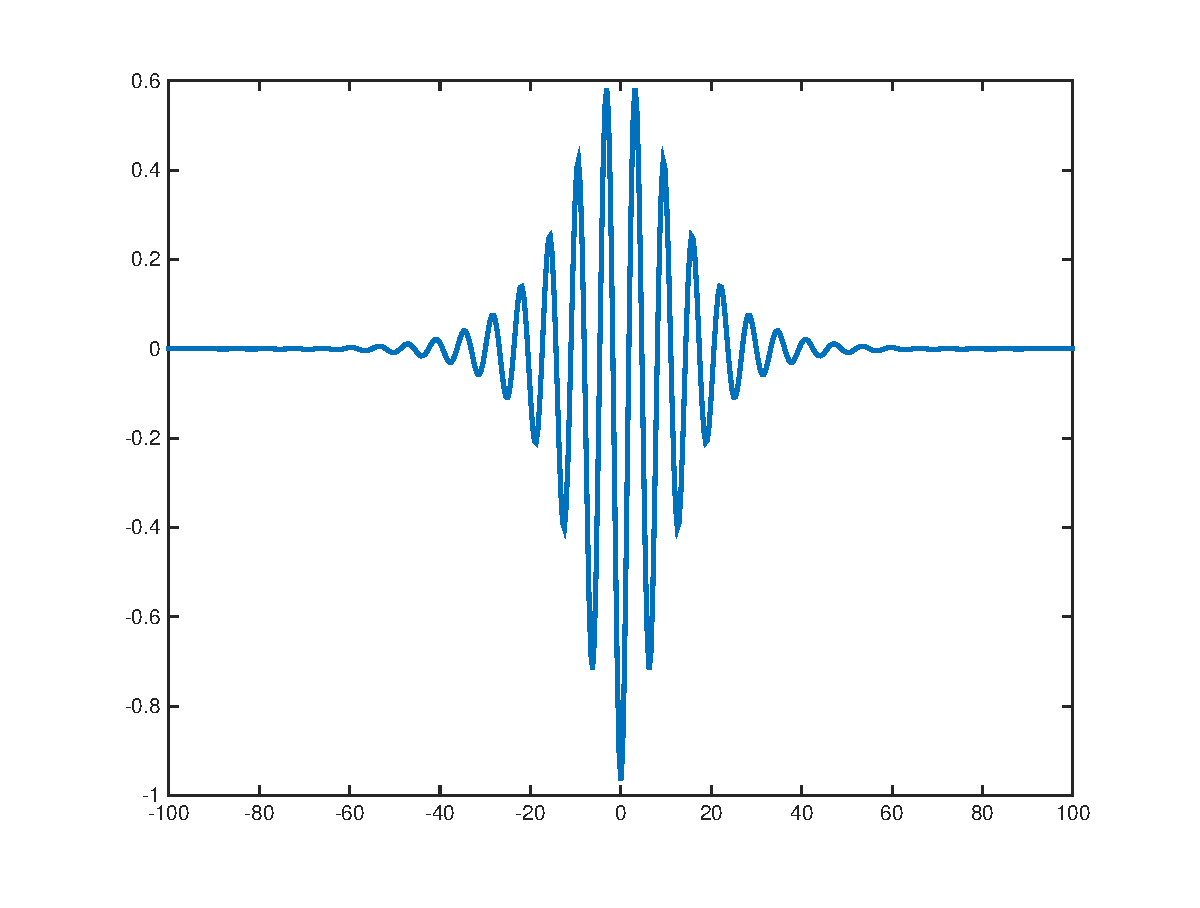
\includegraphics[width=13cm]{images/single14.eps}
          \caption{Primary pulse solutions, $c = 1.354$ (left) and $c = 1.40$ (right).}
          \label{fig:single1}
          \end{center}
          \end{figure}
        }
      \end{block}

      \vskip1ex
   
      \begin{block}{Acknowledgments}
        \small{\rmfamily{This work is supported by the NSF Grant 1148284 }} \\
        \vspace{0.5in}
      \end{block}

    \end{column}

\begin{column}{\sepwid}\end{column}     % empty spacer column

% second column
    \begin{column}{\onecolwid}

      \begin{block}{Multi-Pulse Solutions}
      \rmfamily{
      \textbf{Theorem 2. }(\cite{San97}) Let $q(x)$ be a localized homoclinic orbit solution to \eqref{eqODE}. Choose any integer $n \geq 2$ and any sequence of nonnegative integers $k_1, \dots, k_{n-1}$ with at least one of the $k_j \in \{0, 1 \}$.
      \vskip1ex
      \begin{itemize}
        \item For any sufficiently large integer $m$, there exists a unique $n-$modal solution $q_n(x)$ to \eqref{eqODE}. This solution resembles $n$ well-separated copies of the primary pulse $q(x)$. The distance between successive peaks is $2X_1, \dots, 2X_{n-1}$, where
        \begin{equation*}
        X_j \approx \frac{\pi}{\beta}(2 m + k_j) + C
        \end{equation*}

        \item The linearization of \eqref{eqODE} about $q_n(x)$ is

          \begin{equation*}\label{defA0}
          A_0(q_n) = \partial_x^4 + c^2 \partial_x^2 + e^{q_n}.
          \end{equation*} 

          $A_0(q_n)$ has precisely $n$ real eigenvalues $\nu_j$ close to 0, where $\nu_n = 0$ is a simple eigenvalue. For $j = 1, \dots, n-1$,

          \begin{align*}
          \nu_j < 0 \text{ if } k_j \text{ is odd} \\
          \nu_j > 0 \text{ if } k_j \text{ is even} 
          \end{align*}

        \end{itemize}

        \begin{figure}
        \begin{center}
        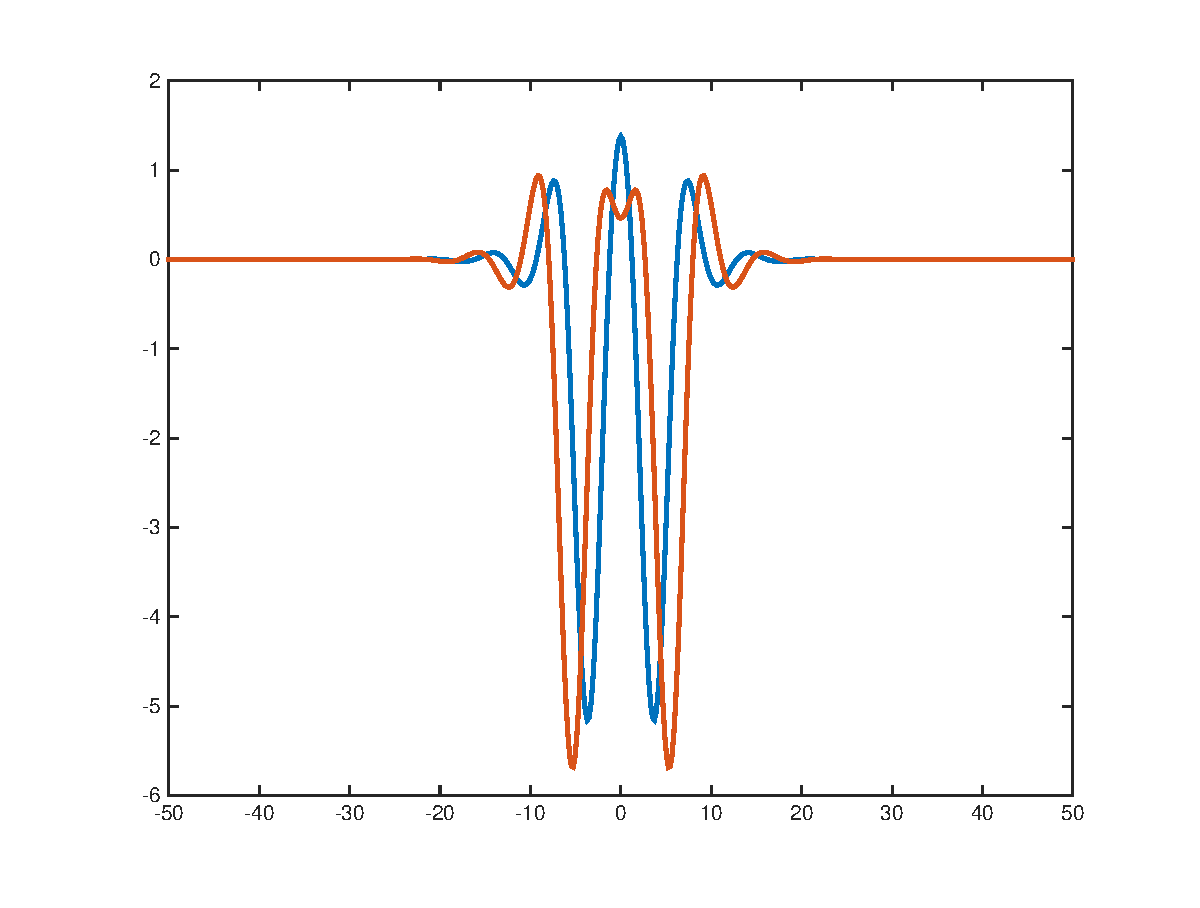
\includegraphics[width=13cm]{images/double12_12.eps}
        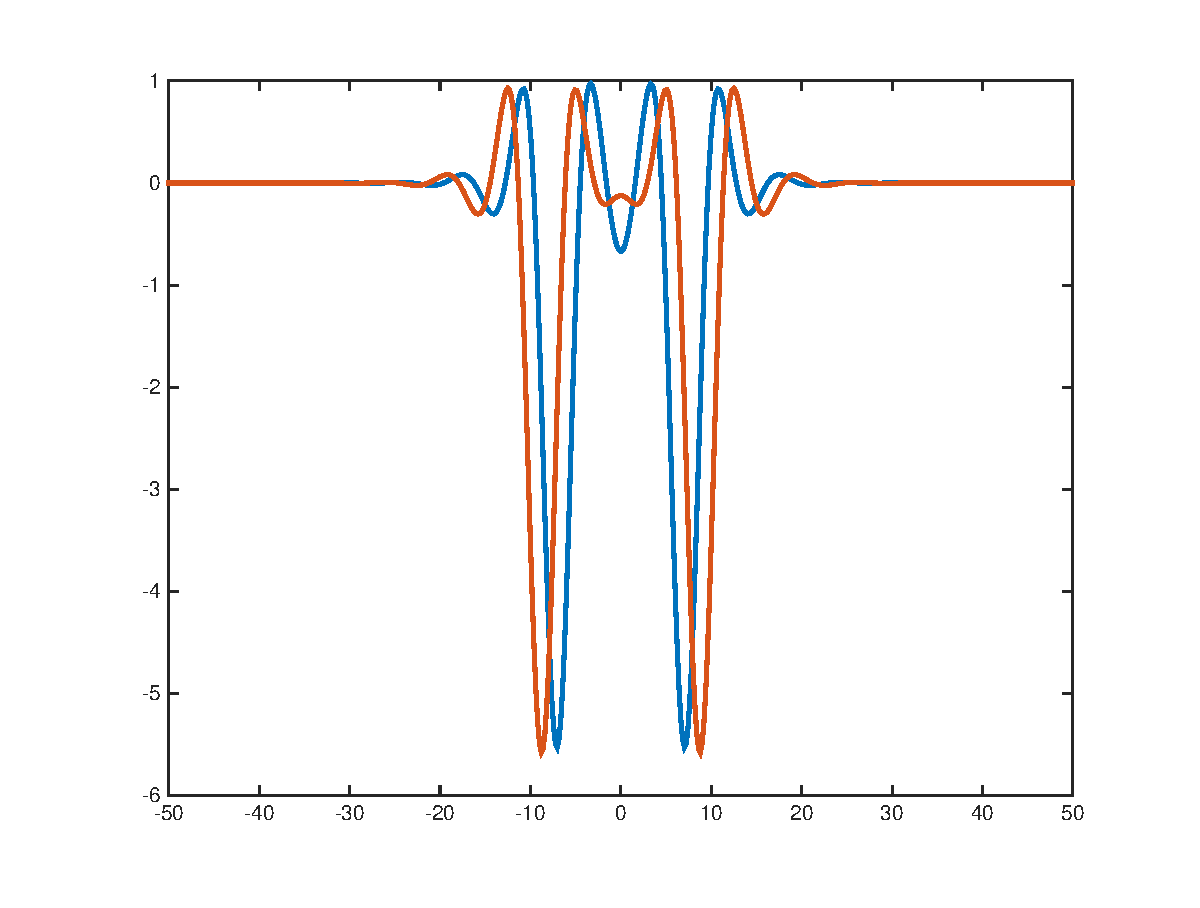
\includegraphics[width=13cm]{images/double12_34.eps}
        \caption{First four 2-pulse solutions to \eqref{eqODE}, $c = 1.2$}
        \label{fig:double}
        \end{center}
        \end{figure}
      }
      \end{block} 

      \vskip1ex

      \begin{block}{PDE Eigenvalue Problem}
      \rmfamily{
      Linearization of the PDE \eqref{PDEc} about the $n-$pulse solution $q_n(x)$ is the quadratic eigenvalue problem

      \begin{equation}\label{quadeig}
      P_2(\lambda; q_n)v =  [A_2 \lambda^2 + A_1 \lambda + A_0(q_n)]v = 0
      \end{equation}

      \begin{align*}
      A_0(q_n) &= \partial_x^4 + c^2 \partial_x^2 + e^{q_n} \\
      A_1 &= -2 c \partial_x \\
      A_2 &= I
      \end{align*}

      }
      \end{block}

    \end{column}

\begin{column}{\sepwid}\end{column}     % empty spacer column

% third column
    \begin{column}{\onecolwid}
      \begin{block}{Essential Spectrum}
        \rmfamily{
          The essential spectrum of \eqref{quadeig} is purely imaginary and is bounded away from the origin.

        }
      \end{block}

      \vskip1ex

      \begin{block}{Krein Matrix}
        \rmfamily{
        Consider a polynomial eigenvalue problem
        \begin{equation}\label{polyeig}
        P_n(\lambda) = \sum_{j=0}^n \lambda_j A_j = 0
        \end{equation}
        where the operators $A_j$ are Hermitian for $j$ even and skew-Hermitian for $j$ odd.\\
        \vskip1ex
        The Krein Matrix is a matrix-valued function $K(\lambda)$ with the properties that for $\lambda \in i\mathbb{R}$
        \vskip1ex
        \begin{itemize}
          \item $K(\lambda)$ is meromorphic
          \item $\det K(\lambda) = 0$ only if $\lambda$ is a polynomial eigenvalue
          \item $K(\lambda)$ can be used to determine the Krein signature of a polynomial eigenvalue
        \end{itemize}
      }
      \end{block}

      \begin{block}{Krein Matrix Construction}
        \rmfamily{

        Let $S$ be the $n-$dimensional space 
        \begin{equation*}\label{defS}
        S = \text{span}\{s_1, \dots, s_n \}
        \end{equation*}

        where $s_j(x)$ are the eigenfunctions corresponding to the small eigenvalues $\nu_j$ from Theorem 2.

        \vskip1ex

        The Krein matrix is the $n\times n$ matrix $K(z)$, where 

        \begin{align}\label{Kreinmatrix}
        [K&(z)]_{jk} = 
        \langle s_j , P_2(iz)s_k\rangle \\
        &- \langle s_j , P_2(iz) P_{S^{\perp}} (P_{S^{\perp}} P_2(iz)|_{S^{\perp}} )^{-1} P_{S^{\perp}} P_2(iz) s_k \rangle \nonumber
        \end{align}

        \vskip1ex

        \textbf{Theorem 3. }Let $q_n(x)$ be an $n-$pulse solution to \eqref{eqODE}. Let $\nu_1, \dots, \nu_n$ be the small eigenvalues of $A_0(q_n)$, as defined in Theorem 2. Then, under some mild hypotheses, the Krein matrix is given by

        \begin{align}\label{Kreinapprox}
        K_S(z) = ||&q_x||^2 \text{diag} (\nu_1, \dots, \nu_n) \\
         &+ d''(c) I \overline{z}^2 + \mathcal{O}(e^{-(3 \alpha/2) X_m}|z| + |z|^3), \nonumber
        \end{align}

        \begin{align*}
        d''(c) &= -\frac{\partial}{\partial c} \left( c ||q_x||^2 \right) \\
        X_m &= \min\{ X_1, \dots, X_{n-1} \} 
        \end{align*}
      }
      \end{block}

  \end{column}

\begin{column}{\sepwid}\end{column}     % empty spacer column

% fourth column
\begin{column}{\onecolwid}

    \begin{block}{Stability Criterion}
    \rmfamily{
    \textbf{Corollary. }Let $q_n(x)$ be an $n-$pulse solution to \eqref{eqODE}, constructed according to Theorem 2 using the sequence of nonnegative integers $\{ k_1, \dots, k_{n-1} \}$ and the nonnegative integer $m$. Let $\nu_1, \dots, \nu_n$ be the small eigenvalues of $A_0(q_n)$, where $\nu_n = 0$.
    \vskip1ex
    \begin{itemize}
      \item If $\nu_1, \dots, \nu_{n-1} < 0$ (equivalently, all $k_j$ are odd), then for sufficiently large $m$, equation \eqref{quadeig} has $n - 1$ pairs of purely imaginary eigenvalues near 0, which are given by

      \begin{equation*}\label{npulseKreineigs}
      \lambda_j^\pm = \pm i \left( ||q_x|| \sqrt{ \frac{|\nu_j|}{d''(c)} } + \mathcal{O}(e^{-(3 \alpha/2) X_m}) \right)
      \end{equation*}

      Thus $q_n(x)$ is linearly neutrally stable.

      \item If $\nu_j > 0$ for some $j = 1, \dots, n-1$ (equivalently, at least one $k_j$ is even), then equation \eqref{quadeig} has at least one eigenvalue with positive real part. Thus $q_n(x; c)$ is linearly unstable.
    \end{itemize}
    
    }
    \end{block}

    \begin{block}{Future Work}
        \rmfamily{
        \begin{itemize}
          \item Explore other applications of the Krein Matrix.
          \item Use Lin's method for stability analysis of multi-pulse solutions to the suspension bridge equation.
        \end{itemize}
        }
      \end{block} 

    \vskip1ex
  
    \begin{block}{References}
      \small{\rmfamily{\begin{thebibliography}{99}
      \bibitem{Chen97} Chen Y. and McKenna P.J. \emph{Traveling Waves in a Nonlinearly Suspended Beam: Theoretical Results and Numerical Observations}. J. Diff. Eq., 136 (1997), 325-355.
      \bibitem{Berg18} van den Berg J.B. et al. \emph{Continuation of homoclinic orbits in the suspension bridge equation: A computer-assisted proof}. J. Diff. Eq., 264 (2018), 3086-3120.
      \bibitem{Chamard11} Chamard J. et al. \emph{Computation of Minimum Energy Paths for Quasi-Linear Problems}. J. Sci. Comp., 49 (2011), 180-194.
      \bibitem{San97} Sandstede B. \emph{Instability of Localized Buckling Modes in a One-Dimensional Strut Model}. Phil. Trans. Roy. Soc. A, 355 (1997), 2083-2097.
      \end{thebibliography}}}

    \end{block}

  \end{column}
  \begin{column}{\sepwid}\end{column}			% empty spacer column
 \end{columns}
\end{frame}
\end{document}
